\documentclass[12pt,xcolor=table,aspectratio=169]{beamer}
\usetheme{Frankfurt}
\usecolortheme{rose}
\usepackage{amsthm}
\usepackage{amsmath}
\usepackage{bbm}
\usepackage{amsfonts}
\usepackage{amssymb}
\usepackage{graphicx}
\usepackage{hyperref}
\usepackage[flushleft]{threeparttable}
\usepackage{tabularx}
\usepackage{booktabs}
\usepackage{siunitx}
\usepackage{tikz}
\usetikzlibrary{decorations.pathreplacing,angles,quotes}
%\usepackage{enumitem}% http://ctan.org/pkg/enumitem

%set up course and number

\newcommand{\ClassName}{TBD}
\newcommand{\ClassNumber}{TBD}
\newcommand{\Topic}{TBD}

% Some optional colors. Change or add as you see fit.
%---------------------------------------------------
 \definecolor{ualbertagreen}{HTML}{007C41}
\definecolor{ualbertagold}{HTML}{FFDB05}

\definecolor{calloutgrey}{HTML}{D9D9D9}


%set fonts
\setbeamerfont{subtitle}{size=\large,shape=\scshape,series=\bfseries}
\setbeamerfont{title}{size=\Large,shape=\scshape,series=\bfseries}
\setbeamerfont{author}{size=\large}
\setbeamerfont{date}{size=\large}
\setbeamerfont{caption}{size=\scriptsize}


% Some optional color adjustments to Beamer. Change as you see fit.
%------------------------------------------------------------------
\setbeamercolor{frametitle}{fg=ualbertagreen,bg=white}
\setbeamercolor{title}{fg=ualbertagreen,bg=white}
\setbeamercolor{author}{fg=ualbertagreen,bg=white}
\setbeamercolor{date}{fg=ualbertagreen,bg=white}
\setbeamercolor{local structure}{fg=ualbertagreen}
\setbeamercolor{section in toc}{fg=ualbertagreen,bg=white}
% \setbeamercolor{subsection in toc}{fg=ualbertagreen,bg=white}
\setbeamercolor{footline}{fg=ualbertagreen!50, bg=white}

% definition boxes
\setbeamercolor{block title}{bg=ualbertagreen,fg=white}
\setbeamercolor{block body}{parent=normal text,use=block title,bg=calloutgrey}
%\setbeamercolor{block body}{parent=normal text,use=block title,bg=block title.bg!30!bg}


\setbeamercolor{upper separation line head}{bg=ualbertagreen}
\setbeamercolor{lower separation line head}{bg=ualbertagold}
\setbeamercolor{middle separation line head}{bg=ualbertagold}
\setbeamercolor{frametitle}{fg=ualbertagreen,bg=white}



\setbeamercolor{section in head/foot}{bg=white,fg=ualbertagreen}
\setbeamercolor{author in head/foot}{bg=white,fg=ualbertagreen}
\setbeamercolor{date in head/foot}{bg=white,,fg=ualbertagreen}
\setbeamercolor{title in head/foot}{bg=white,fg=ualbertagreen}

\setbeamercolor{headline}{bg=white,fg=ualbertagreen}




\setbeamercolor*{middle separation line head}{bg=ualbertagreen}
\setbeamercolor*{alerted text}{fg=black}
\setbeamerfont{alerted text}{series=\bfseries}
\setbeamercolor*{example text}{fg=black}
\setbeamercolor*{structure}{fg=black}


\let\Tiny=\tiny



\logo{
   %\ifnum\insertpagenumber>1
   \tikz [remember picture,overlay]
    \node[yshift=.3cm,xshift=1.5cm] at (current page.south west)
        %or: (current page.center)
        {
\includegraphics[width=1in]{../images/UA-ASB-COLOUR.png}};
    %\fi
%
\includegraphics[height=0.8cm]{../images/UA-ASB-COLOUR.png}\vspace{220pt}
}


\setbeamertemplate{title page}{%
  \vbox{}
    \vspace{.5cm}% NEW
  \begingroup
    \centering
    \begin{beamercolorbox}[sep=8pt,center]{title}
      \usebeamerfont{title}\ClassNumber: \ClassName\par%
      \usebeamerfont{title}\inserttitle\par%
     \ifx\insertsubtitle\@empty%
      \else%
        \vskip0.05em%
        {\usebeamerfont{subtitle}\usebeamercolor[fg]{subtitle}\insertsubtitle\par}%
      \fi%
    \end{beamercolorbox}%
    \begin{beamercolorbox}[sep=8pt,center]{author}
      \usebeamerfont{author}\insertauthor
    \end{beamercolorbox}
    \begin{beamercolorbox}[sep=8pt,center]{institute}
      \usebeamerfont{institute}\insertinstitute
    \end{beamercolorbox}

    \vspace{0.5cm}% NEW
    \begin{beamercolorbox}[sep=8pt,center]{date}
      \usebeamerfont{date}\insertdate
    \end{beamercolorbox}\vskip0.05em

      \endgroup
  %\vfill
}


\setbeamertemplate{frametitle}{%
    \insertframetitle\par\vskip-10pt
}



\renewcommand{\ClassName}{Business Economics, Organization and Management}
\renewcommand{\ClassNumber}{BUEC 311}

\setbeamertemplate{headline}{%
\leavevmode%
 \hbox{%
    \begin{beamercolorbox}[wd=\paperwidth,ht=5ex,dp=0ex]{white}%
    \usebeamerfont{headline}\hskip6pt\ClassNumber: \inserttitle\par%
    \insertsectionnavigationhorizontal{\paperwidth}{}{\hskip0pt plus1filll}
    \end{beamercolorbox}%
  }
}

\defbeamertemplate*{footline}{my footline}{%
    \ifnum\insertpagenumber=1
        \Tiny{%
            \hfill%
		\vspace*{1pt}%
            %\insertframenumber/\inserttotalframenumber \hspace*{0.1cm}%
            \newline%
            \color{ualbertagold}{\rule{\paperwidth}{0.4mm}}\newline%
            \color{ualbertagold}{\rule{\paperwidth}{.4mm}}%
        }
  \else%
        \Tiny{%
            \hspace{.66\paperwidth}
            %\vspace{25pt}
            \insertframenumber/\inserttotalframenumber
            \newline%
            \color{ualbertagold}{\rule{\paperwidth}{0.4mm}}\newline%
            \color{ualbertagold}{\rule{\paperwidth}{.4mm}}%
        }%
    \fi%
}


\newenvironment{itemize*}%
  {\begin{itemize}%
    \setlength{\itemsep}{0pt}%
    \setlength{\parskip}{0pt}}%
  {\end{itemize}}


\title{
Monopoly
}

\date{Fall 2020}

\begin{document}

\section{Outline}

\frame{
	\titlepage
}

\frame{
	\frametitle{Outline}
	\begin{enumerate}
	\item Monopoly Profit Maximization
	\item[]
	\item Market Power
	\item[]
	\item Market Failure Due to Monopoly Pricing
	\item[]
	\item Causes of Monopoly
	\item[]
	\item Advertising
	\item[]
	\item Networks, Dynamics \& Behavioural Economics
	\end{enumerate}
}

\section{Monopoly Profit Maximization}

\frame{
	\frametitle{Outline}
	\begin{enumerate}
	\item \alert{Monopoly Profit Maximization}
	\item[]
	\item Market Power
	\item[]
	\item Market Failure Due to Monopoly Pricing
	\item[]
	\item Causes of Monopoly
	\item[]
	\item Advertising
	\item[]
	\item Networks, Dynamics \& Behavioural Economics
	\end{enumerate}
}

\frame{
	\frametitle{Monopoly Profit Maximization}
	\begin{itemize}
	\item \underline{Monopoly:} Sole supplier of a good for which there is no close substitute.
	\item[]
	\item Like a perfectly competitive firm, a monopoly maximizes profit by setting $MR(q) = MC(q)$.
	\item[]
	\item Key difference: Because a monopoly has no competitors, it faces a downward-sloping market demand curve.
		\begin{itemize}
		\item This means a monopoly can alter its revenue by changing the price that it charges.
		\item But there is a trade-off from lowering price.
			\begin{itemize}
			\item More demand vs. lower price.
			\end{itemize}
		\end{itemize}
	\end{itemize}
}

\frame{
	\frametitle{Monopoly Profit Maximization}
	\begin{figure}
	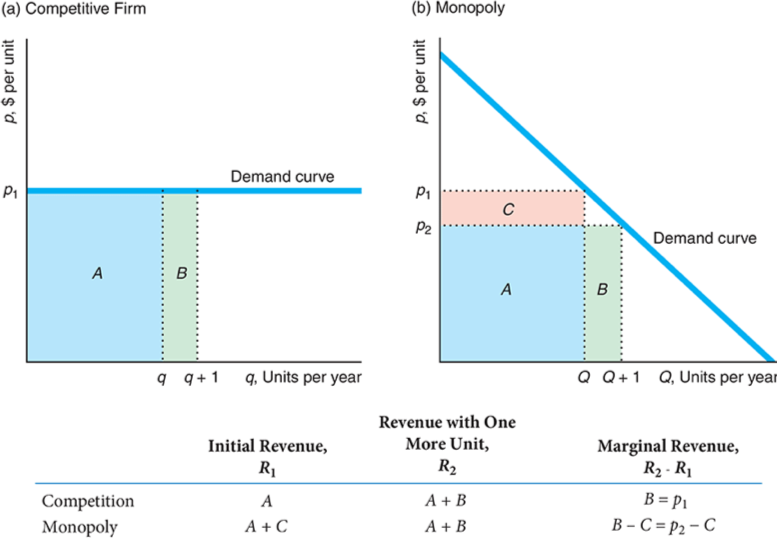
\includegraphics[scale=0.66]{../images/monopoly/pc_v_m_revenue.png}
	\end{figure}
}

\frame{
	\frametitle{Price vs. Marginal Revenue}
	\begin{itemize}
	\item A monopoly's marginal revenue from selling an additional unit must be less than the price of the unit.
	\item[]
	\item This means that the monopolist's $MR$ curve will lie below the demand curve for any possible $Q$, and the shape of the $MR$ curve will depend on the shape of the demand curve.
	\item[]
	\item In general:
		\begin{align*}
		MR = p + \left[\frac{\Delta p}{\Delta Q}\right] Q
		\end{align*}
		where $\Delta p/\Delta Q <0$.
	\end{itemize}
}

\frame{
	\frametitle{Elasticity of Demand}
	\begin{itemize}
	\item We can describe the shape of the demand curve at a particular quantity with the \underline{price elasticity of demand}:
		\begin{align*}
		\varepsilon = \frac{[\Delta Q/Q]}{[\Delta p/p]}<0
		\end{align*}
	\item[]
	\item $\varepsilon$ indicates the percentage change in quantity demand from a 1\% change in price.
	\item[]
	\item If demand is \textit{inelastic}, $-1 < \varepsilon \leq 0$.
	\item If demand is \textit{elastic}, $\varepsilon < -1$.
	\end{itemize}
}

\frame{
	\frametitle{Marginal Revenue and Elasticity}
	\begin{itemize}
		\item We can rewrite the monopolist's marginal revenue function in terms of the price elasticity of demand:
		\begin{align*}
		MR & = p + \left[\frac{\Delta p}{\Delta Q} \right]Q\\
			& = p + p \left[\frac{\Delta p}{\Delta Q} \right] \frac{Q}{p}\\
			& = p \left[ 1 + \frac{1}{[\Delta Q/Q]/[\Delta p/p]} \right]\\
			& = p \left[1 + \frac{1}{\varepsilon} \right]
		\end{align*}
	\end{itemize}
}

\frame{
	\frametitle{Marginal Revenue}
	\begin{figure}
	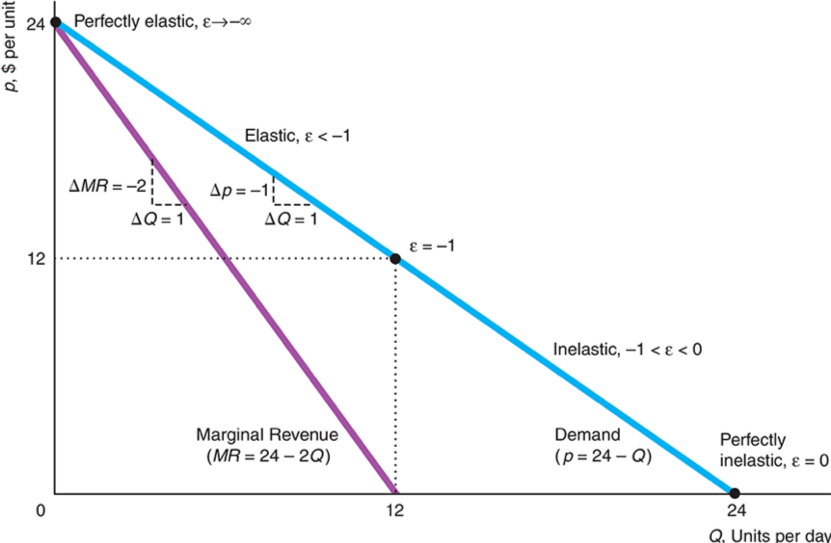
\includegraphics[scale=0.66]{../images/monopoly/demand_mr.png}
	\caption{Demand and Marginal Revenue for p=24-Q}
	\end{figure}
}

\frame{
	\frametitle{Marginal Revenue}
	\begin{figure}
	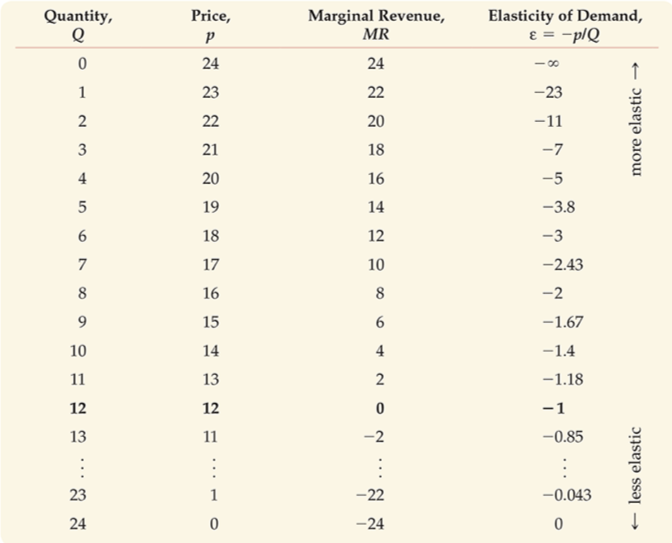
\includegraphics[scale=0.66]{../images/monopoly/demand_mr_table.png}
	\caption{Demand and Marginal Revenue for p=24-Q}
	\end{figure}
}

\frame{
	\frametitle{Monopoly Profit Maximization}
	\begin{itemize}
	\item A monopolist maximizes profit such that $MR(Q)=MC(Q)$.
	\item[]
	\item This can be achieved by adjusting price \underline{or} quantity.
		\begin{itemize}
		\item The other variable is determined by the demand curve.
		\end{itemize}
	\item[]
	\item Here, we will focus on the case when the monopolist sets quantity.
	\end{itemize}
}

\frame{
	\frametitle{Two-Step Analysis}
	\begin{itemize}
	\item Monopolists also use two-step analysis to maximize profit.
	\item[]
	\item Step 1: Choose $Q$ to maximize profit.
		\begin{itemize}
		\item This occurs where $MR(Q)=MC(Q)$.
		\end{itemize}
	\item[]
	\item Step 2: Decide whether to produce or shut down.
		\begin{itemize}
		\item Short run: Shut down if price is less than average variable cost.
		\item Long run: Shut down if price is less than average cost.
		\end{itemize}
	\end{itemize}
}

\frame{
	\frametitle{Monopoly Profit Maximization}
	\begin{figure}
	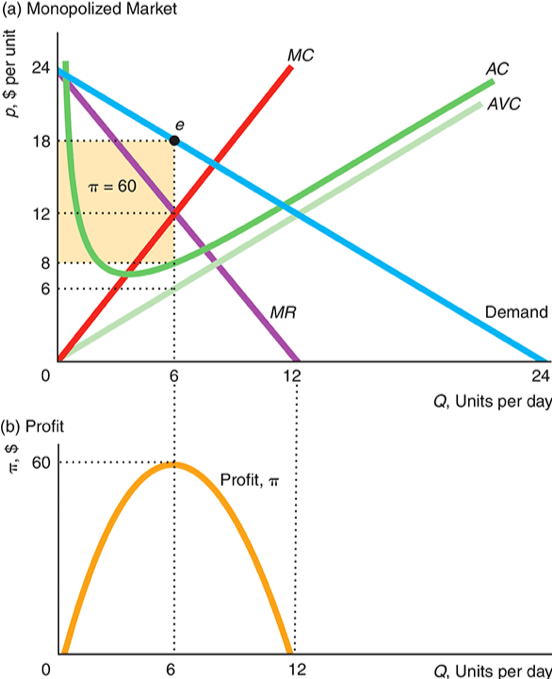
\includegraphics[scale=0.66]{../images/monopoly/m_pi_max.png}
	\end{figure}
}

%\frame{
	%\frametitle{Demand Changes}
	%\begin{itemize}
	%\item In a perfectly competitive market, the effect of a shift in demand on a firm's output depends only on the shape of the marginal cost curve.
	%\item[]
	%\item In a monopoly, the effect of a shift in demand on firm's output depends on shape of the marginal cost curve, \textit{and on the shape of the demand curve}.
%		\begin{itemize}
%		\item Unlike a competitive firm, a monopoly does not have a well defined supply curve.
%		\end{itemize}
	%\end{itemize}
%}

%\frame{
	%\frametitle{Demand Changes}
	%\begin{figure}
	%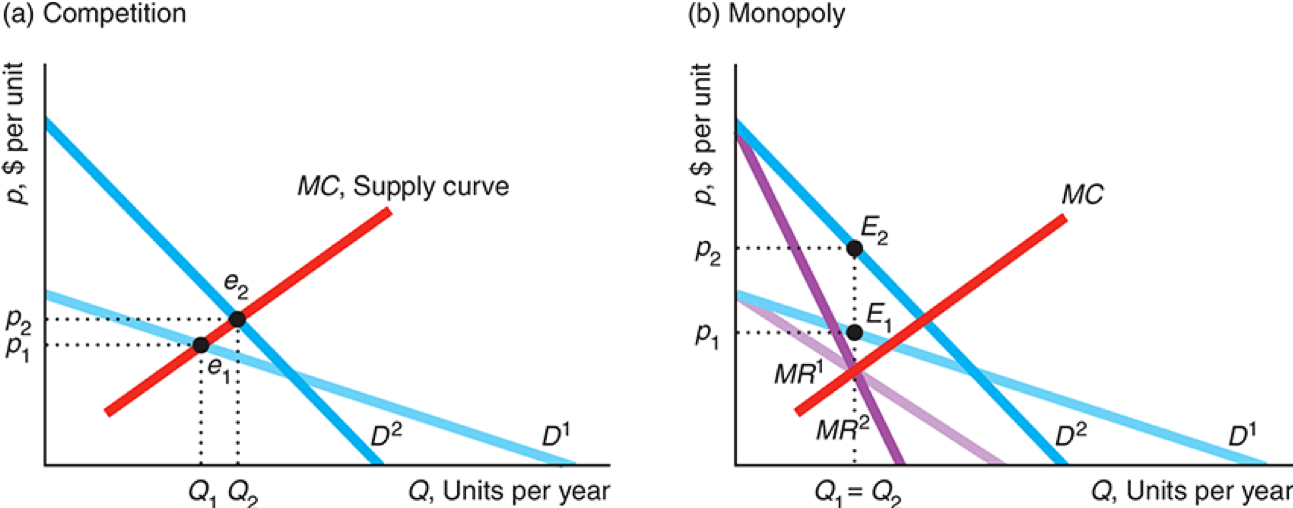
\includegraphics[scale=0.66]{../images/monopoly/no_supply.png}
	%\end{figure}
%}
\section{Market Power}

\frame{
	\frametitle{Outline}
	\begin{enumerate}
	\item Monopoly Profit Maximization
	\item[]
	\item \alert{Market Power}
	\item[]
	\item Market Failure Due to Monopoly Pricing
	\item[]
	\item Causes of Monopoly
	\item[]
	\item Advertising
	\item[]
	\item Networks, Dynamics \& Behavioural Economics
	\end{enumerate}
}

\frame{
	\frametitle{Market Power}
	\begin{itemize}
	\item \underline{Market Power}: A firm's ability to affect the market price.
	\item[]
	\item The shape of the demand curve constraints a monopoly's ability to exercise market power.
	\item[]
	\item To see this, note that profit maximization implies:
		\begin{align*}
		\frac{p}{MC} = \left[\frac{1}{1+[1/\varepsilon]} \right]
		\end{align*}
	\item[]
	\item Hence, a monopoly's markup increases as demand becomes more inelastic.
	\end{itemize}
}

\frame{
	\frametitle{Market Power}
	\begin{itemize}
	\item We can also measure a firm's market power using the \underline{Lerner Index}, which is given by:
		\begin{align*}
		LI = \frac{p-MC}{p}
		\end{align*}
	\item[]
	\item This can be re-expressed in terms of the elasticity of demand:
		\begin{align*}
		LI = \frac{p-MC}{p} = - \frac{1}{\varepsilon}
		\end{align*}
	\item[]
	\item For a monopoly, the Lerner Index ranges between 0 and 1.
	\end{itemize}
}

\frame{
	\frametitle{Market Power}
	\begin{figure}
	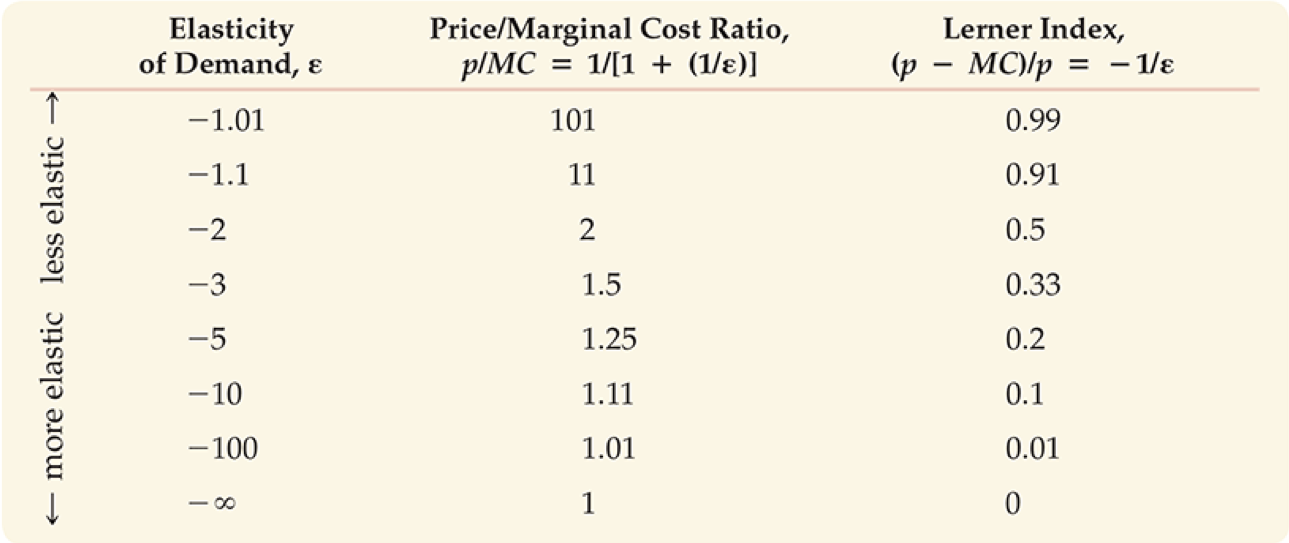
\includegraphics[scale=0.66]{../images/monopoly/mkt_power.png}
	\end{figure}
}

\frame{
	\frametitle{Market Power}
	\begin{itemize}
	\item Firms can exploit the relationship between mark-ups and the elasticity of demand to ensure profits are being maximized.
	\item[]
	\item Recall, if profit is maximized:
		\begin{align*}
		\frac{p}{MC} = \left[\frac{1}{1+[1/\varepsilon]} \right]
		\end{align*}
	\item[]
	\item Hence, with an estimate of $\varepsilon$, firms can ensure that $p/MC$ is approximately equal to $1/[1+[1/\varepsilon]]$. If it is not, then prices need to be adjusted.
	\end{itemize}
}

\frame{
	\frametitle{Market Power}
	\begin{itemize}
	\item Market power is determined by the availability of substitutes, the number of firms in the market, and the proximity of competitors.
		\begin{itemize}
		\item These factors all affect the elasticity of demand.
		\end{itemize}
	\item[]
	\item Market power is lower if:
		\begin{enumerate}
		\item \underline{There are better substitutes}: better substitutes $\implies$ demand is more elastic.
		\item \underline{There are more firms}: more firms provides more choice for consumers $\implies$ demand is more elastic.
		\item \underline{Competitors locate nearby}: nearby competitors $\implies$ demand is more elastic.
		\end{enumerate}
	\end{itemize}
}

\section{Monopoly Pricing}

\frame{
	\frametitle{Outline}
	\begin{enumerate}
	\item Monopoly Profit Maximization
	\item[]
	\item Market Power
	\item[]
	\item \alert{Market Failure Due to Monopoly Pricing}
	\item[]
	\item Causes of Monopoly
	\item[]
	\item Advertising
	\item[]
	\item Networks, Dynamics \& Behavioural Economics
	\end{enumerate}
}

\frame{
	\frametitle{Market Failure Due to Monopoly Pricing}
	\begin{itemize}
	\item \underline{Recall}: Perfect competition achieves \textit{economic efficiency}.
		\begin{itemize}
		\item Perfect competition maximizes total surplus.
		\end{itemize}
	\item[]
	\item A monopoly is \textit{economically inefficient}.
		\begin{itemize}
		\item A monopolist sets prices above marginal cost, so consumers buy less than the efficient level of the good or service.
		\item This wastes potential surplus, resulting in deadweight loss.
		\item Deadweight loss is inefficient.
		\end{itemize}
	\item[]
	\item The inefficiency created by monopoly is an example of a \underline{market failure}.
		\begin{itemize}
		\item A market failure is a non-optimal allocation of goods and services.
		\end{itemize}
	\end{itemize}
}

\frame{
	\frametitle{Market Failure Due to Monopoly Pricing}
	\begin{figure}
	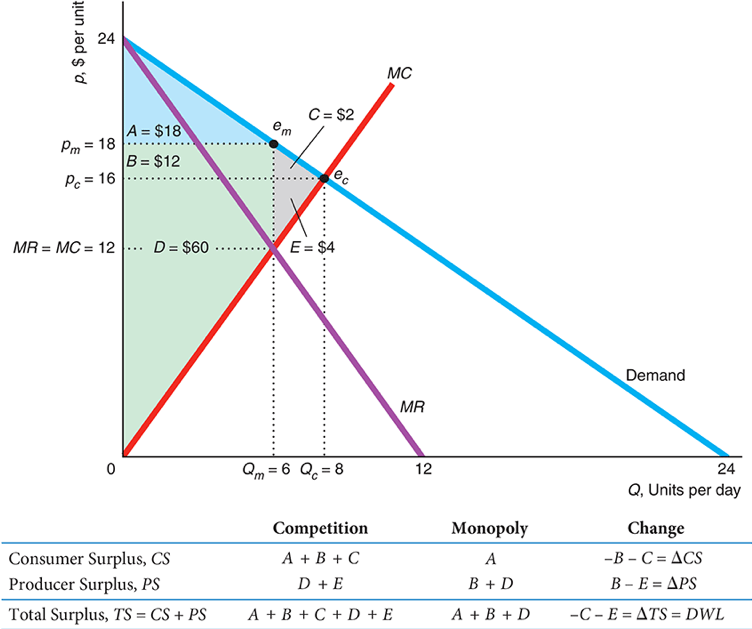
\includegraphics[scale=.6]{../images/monopoly/dwl_monopoly.png}
	\caption{The Deadweight Loss from Monopoly}
	\end{figure}
}


\frame{
	\frametitle{Outline}
	\begin{enumerate}
	\item Monopoly Profit Maximization
	\item[]
	\item Market Power
	\item[]
	\item Market Failure Due to Monopoly Pricing
	\item[]
	\item \alert{Causes of Monopoly}
	\item[]
	\item Advertising
	\item[]
	\item Networks, Dynamics \& Behavioural Economics
	\end{enumerate}
}

\section{The Causes of Monopoly}

\frame{
	\frametitle{The Causes of Monopoly}
	\begin{itemize}
	\item Monopolies arise from two main factors:
		\begin{enumerate}
		\item Cost considerations.
		\item[]
		\item Government policy.
		\end{enumerate}
	\end{itemize}
}

\frame{
	\frametitle{The Causes of Monopoly}
	\begin{itemize}
	\item Cost-based monopolies can be due to:
		\begin{itemize}
		\item \underline{Cost advantages}: One firm has substantially lower costs than potential rivals.
			\begin{itemize}
			\item The low-cost firm will be able to function as a monopoly if it is able to sell at a price so low that potential rivals would lose money if they enter the market.
			\item These cost advantages can arise due to superior technology, better production methods, or control of an essential facility/scare resource.
			\end{itemize}
		\item[]
		\item \underline{Natural monopoly}: One firm is able to produce total market output at a lower cost than two or more firms could.
			\begin{itemize}
			\item That is: $C(Q) < C(q_{1}) + C(q_{2}) + \ldots + C(q_{N})$.
			\item This can occur due to economies of scale; a natural monopolist will have a strictly declining average cost curve.
			\item Governments use the natural monopoly argument to justify granting monopoly rights to public utilities.
			\end{itemize}
		\end{itemize}
	\end{itemize}
}

\frame{
	\frametitle{Natural Monopoly}
	\begin{figure}
	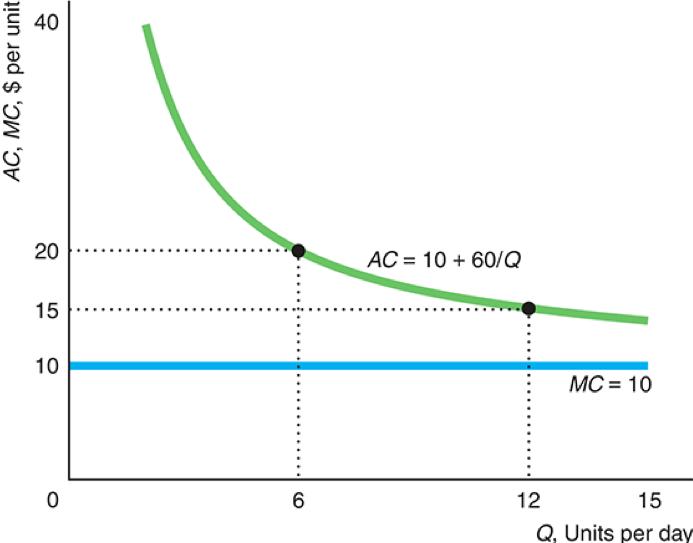
\includegraphics[scale=.6]{../images/monopoly/natural_m.png}
	\caption{Natural Monopoly}
	\end{figure}
}

\frame{
	\frametitle{Government-created Monopoly}
	\begin{itemize}
	\item Monopolies can also arise as a result of governments:
		\begin{itemize}
		\item Creating \underline{barriers to entry}.
			\begin{itemize}
			\item Governments can require firms to obtain a license to operate, or explicitly grant monopoly rights to a single firm.
			\item If the government auctions off the monopoly rights, it can potentially capture the value of monopoly earnings. However, for political and other reasons, the government usually does not capture all future profits.
			\end{itemize}
		\item[]
		\item Granting \underline{patents}.
			\begin{itemize}
			\item Patents are exclusive rights granted to a patent holder for a specified length of time.
			\item Patents only granted for new and useful product, process, substance or design.
			\item Patent lengths vary across countries. Typically 20 years in both Canada and United States.
			\end{itemize}
		\end{itemize}
	\end{itemize}
}
\section{Advertising}

\frame{
	\frametitle{Outline}
	\begin{enumerate}
	\item Monopoly Profit Maximization
	\item[]
	\item Market Power
	\item[]
	\item Market Failure Due to Monopoly Pricing
	\item[]
	\item Causes of Monopoly
	\item[]
	\item \alert{Advertising}
	\item[]
	\item Networks, Dynamics \& Behavioural Economics
	\end{enumerate}
}

\frame{
	\frametitle{Advertising}
	\begin{itemize}
	\item Unlike a perfectly competitive firm, a monopolist has an incentive to try and alter demand for its product via advertising.
	\item[]
	\item Goal of advertising: shift the demand curve outward and make it less elastic.
		\begin{itemize}
		\item This means the monopolist can sell more units a higher price.
		\end{itemize}
	\item[]
	\item A monopolist should only advertise if it expects \underline{net profit} (profit minus the cost of advertising) to increase.
		\begin{itemize}
		\item If the monopolist advertises, the quantity of advertising should be chosen such that the marginal benefit (the marginal revenue from additional unit sold) equals the marginal cost.
		\end{itemize}
	\end{itemize}
}

\frame{
	\frametitle{Advertising}
	\begin{figure}
	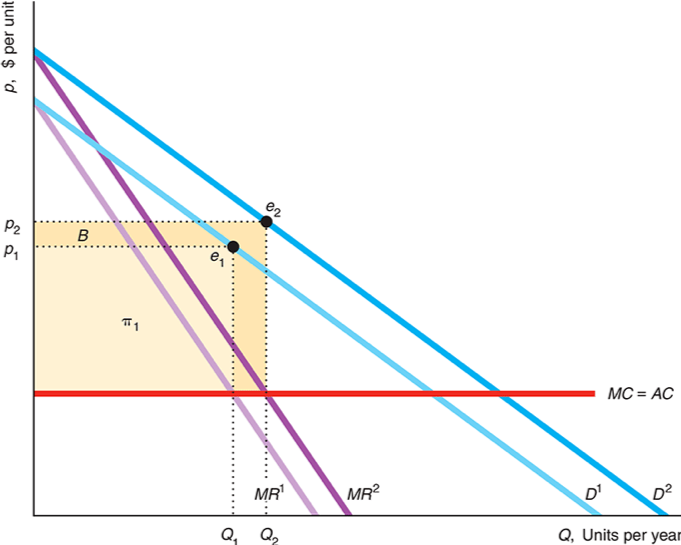
\includegraphics[scale=0.66]{../images/monopoly/advertising.png}
	\end{figure}
}

\section{Dynamic Incentives}


\frame{
	\frametitle{Outline}
	\begin{enumerate}
	\item Monopoly Profit Maximization
	\item[]
	\item Market Power
	\item[]
	\item Market Failure Due to Monopoly Pricing
	\item[]
	\item Causes of Monopoly
	\item[]
	\item Advertising
	\item[]
	\item \alert{Networks, Dynamics \& Behavioural Economics}
	\end{enumerate}
}

\frame{
	\frametitle{Networks, Dynamics \& Behavioural Economics}
	\begin{itemize}
	\item In some settings, the decisions of a monopolist are inherently dynamic due to the presence of network externalities in demand.
	\item[]
	\end{itemize}
	\begin{definition}[Network Externality]
	A good exhibits a network externality if one consumer's demand depends on the consumption of the good by others.
	\end{definition}
	\begin{itemize}
	\item[]
	\item If a network externality is:
		\begin{itemize}
		\item positive,  the value to consumers grows as the number of units sold increases.
		\item negative, the value to consumers falls as the number of units sold increases.
		\end{itemize}
	\end{itemize}
}

\frame{
	\frametitle{Networks, Dynamics \& Behavioural Economics}
	\begin{itemize}
	\item Many industries exhibit positive network externalities because consumers get a direct benefit from a larger network.
		\begin{itemize}
		\item E.g. ATMs, Fax Machines
		\end{itemize}
	\item[]
	\item Firms can also benefit indirectly from network externalities because they offer products that are complementary to a good or service that requires a network.
		\begin{itemize}
		\item E.g. Software, ``YouTubers''
		\end{itemize}
	\end{itemize}
}

\frame{
	\frametitle{Networks, Dynamics \& Behavioural Economics}
	\begin{itemize}
	\item The magnitude of network externalities can depend in part on human psychology, particularly due to consumer attitudes towards other consumers.
	\item[]
	\item Positive network externalities can arise because of \textit{Bandwagon Effects}.
		\begin{itemize}
		\item Individuals place greater value on a good when more people posses it.
		\end{itemize}
	\item[]
	\item Negative network externalities can arise because of \textit{Snob Effects}.
		\begin{itemize}
		\item Individuals place less value on a good when more people posses it.
		\end{itemize}
	\end{itemize}
}

\frame{
	\frametitle{Networks, Dynamics \& Behavioural Economics}
	\begin{itemize}
	\item Positive network externalities can lead to a monopoly because a critical mass of consumers is needed.
	\item[]
	\item One large firm can end up dominating the market.
		\begin{itemize}
		\item E.g. Windows OS; Youtube.
		\end{itemize}
	\item[]
	\item But domination does not necessarily last forever.
		\begin{itemize}
		\item E.g. Yahoo and Google; Netscape, Internet Explorer, and Chrome.
		\end{itemize}
	\end{itemize}
}

\frame{
	\frametitle{Takeaways}
	\begin{enumerate}
	\item A profit maximizing monopolist earns positive profit by choosing its output to equate marginal revenue and marginal costs.
	\item[]
	\item Market power depends on the shape of the demand curve.
	\item[]
	\item Monopoly leads to market failure.
	\item[]
	\item Monopolies can arise due to cost advantages, government policy and network effects.
	\item[]
	\item Advertising can increase the profits of a monopolist.
	\end{enumerate}
}

\end{document}
